\section*{Part 3. Experiments -- predict votes of surveys}

In these experiments, we will apply online convex optimization algorithms to pairwise comparison datasets. Comparison data arises in many different applications such as sport competition, recommender systems or web clicks. We consider the following sequential setting. Let $\Zcal = \{1,\dots,N\}$ be a finite set of items (for example football teams in a competition).

\medskip
At each iteration $t\geq 1$, 
\begin{itemize}[topsep=-2pt]
	\item the learner receives the labels of two items that are competing $z_t = (z_t(1),z_t(2)) \in \Zcal^2$
	\item the learner predicts $\hat y_t \in (0,1)$ the probability of victory of item $z_t(1)$. 
	\item the environment reveals the result of the match $y_t = 1$ if item $z_t(1)$ wins the match and $y_t = 0$ otherwise (if team $z_t(2)$ wins).
\end{itemize}
The learner aims at minimizing his cumulative loss: $\hat L_T = \sum_{t=1}^T \ell(\hat y_t,y_t)$, where 
$
	\ell(\hat y_t,y_t) = (1-\hat y_t) y_t + \hat y_t (1-y_t) 
$.

\begin{enumerate}[resume]
	\item Justify the choice of $\ell$.

\begin{solution}
When dealing with a classification problem like this one, a natural choice would be to minimize the cross-entropy. However, because the definition involves a logarithm, this loss may not be smooth enough for the algorithms we want to use, such as the Online Gradient Descent which requires the loss to have a bounded gradient. Hence, we use a similar but smoother loss, as defined above, to solve this classification problem.
\end{solution}
\end{enumerate}


	\paragraph{Datasets} We consider two datasets from~\cite{salganik2015wiki} that contain surveys of civic comparisons (can be download at \url{http://pierre.gaillard.me/teaching/mva}). Each dataset consists of two files of $T=15\,000$ rows corresponding to votes:
	\begin{itemize}
		\item ideas dataset: the participants are suggested two politic ideas such as ('free beer' vs 'free ice cream') and are asked to vote for the best. 
		\item politicians dataset: the participants are asked  which political figure within a pair such as ('Obama' vs 'Goldman Sachs') had ``the worse year in Washington.''
	\end{itemize}
	The datasets contain two files: 
	\begin{itemize}
		\item \texttt{ideas-id.csv} (resp. \texttt{politicans-id.csv}) that contains id and text of the ideas (resp. political figures). 
		\item \texttt{ideas-votes.csv} (resp. \texttt{politicians-votes.csv}) that contains the id of the two competing ideas (resp. political figures) in z1 and z2 and a column $y$ which is 1 if the participant voted for z1 and 0 otherwise.
	\end{itemize}
	The goal of the learner is to sequentially predict the results of the votes minimizing the number of mistakes.

\begin{enumerate}[resume]
	\item Implement the Exponentially Weighted Average Forecaster (EWA) and Online Gradient Descent (OGD) (and optionally the Prod forecaster of question 1)  with parameter $\eta >0$ that at each round $t\geq 1$ take a finite set of predictions $f_t(1),\dots, f_t(K) \in [0,1]^K$ and forecast $\hat y_t = \sum_{k=1}^K p_t(k) f_t(k) \in [0,1]$ the probability that idea 1 wins the vote. \footnote{This question does not require any answer in the final report. $f_t(1),\dots,f_t(K)$ are prediction of experts that are inputs, they will be defined explicitely in the next question.}

	For the euclidean projection onto the simplex, see~\cite{duchi2008efficient}.

\begin{solution}
 See the code for the implementation details.  
\end{solution}

	\item We consider the sleeping strategies indexed by $k \in \{1,\dots,2N\}$ that predict for $1\leq k\leq N$
	\begin{equation*}
		 \qquad f_t(k) = \left\{ 
			\begin{array}{cc}
				1 & \text{if } k = z_t(1) \\
				0 & \text{if } k = z_t(2) \\
				\emptyset & \text{otherwise}
			\end{array}
		\right. \qquad \text{and} \qquad f_t(k+N) =  \left\{ 
			\begin{array}{cc}
				0 & \text{if } k = z_t(1) \\
				1 & \text{if } k = z_t(2) \\
				\emptyset & \text{otherwise}
			\end{array}
		\right. \,,
	\end{equation*}
	where $\emptyset$ means that the strategy is sleeping.
	Basically, $f_t(k)$ (resp. $f_t(k+N)$) predicts always the victory (resp. loss) of the idea $k$ during the votes. Remark that the sleeping trick of question 2) works for any algorithm so that we might replace $\emptyset$ with the prediction of the algorithm itself $\hat y_t$. Run the two algorithms of the preceding question (EWA, OGD) with these predictions  $f_t(1),\dots, f_t(K) \in [0,1]^K$. 

	\begin{enumerate}[label=(\alph*)]
		\item Plot the cumulative loss of the algorithms at $T = 15\,000$ according to different values of $\eta \in (0,1/2)$ chosen in a grid.
	
	In this question, we plot the cumulative loss for different values of $\eta$, computes with the OGD update and the EWA update.
	
	\begin{solution}
	    \begin{figure}[h!]
    \centering
    \begin{subfigure}{.47\textwidth}
      \centering
      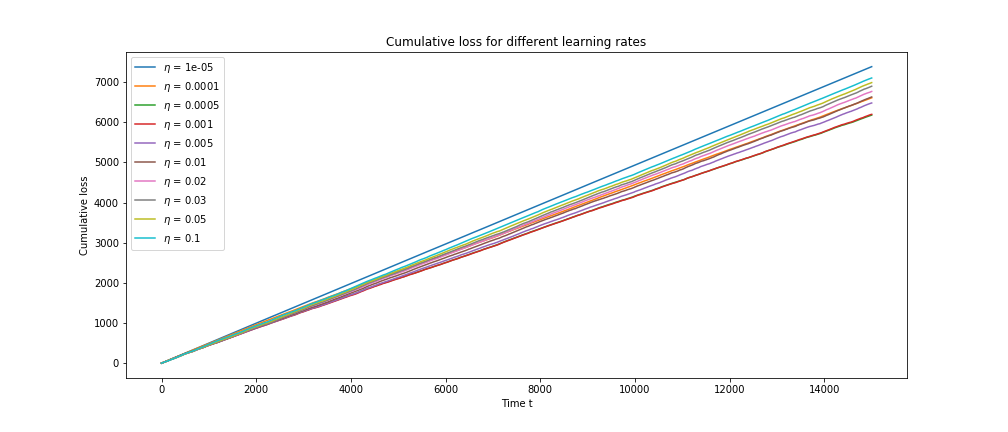
\includegraphics[height=110pt]{image1/image2/VOTES_OGD_cumulative_loss.png}
      \caption{Cumulative loss when playing OGD for different $\eta$ values}
      \label{fig:q7a}
    \end{subfigure}%
    \hspace{2mm}
    \begin{subfigure}{.47\textwidth}
      \centering
      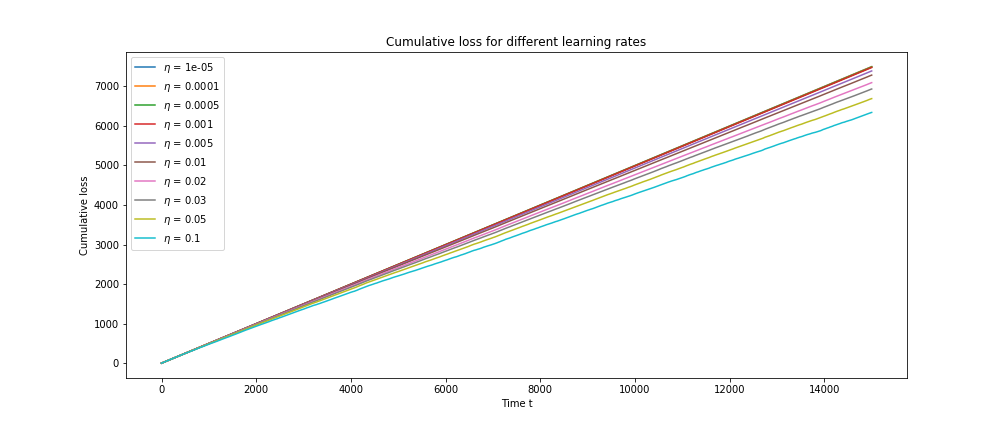
\includegraphics[height=110pt]{image1/image2/VOTES_EWA_cumulative_loss.png}
      \caption{Cumulative loss when playing EWA for different $\eta$ values}
      \label{fig:q7b}
    \end{subfigure}%
    \caption{}
    \end{figure}
	\end{solution}

In both case, the best cumulative loss is obtained for $\eta = 0.001$. However, it is not the value of $\eta = \sqrt{\frac{log(K)}{T}}=0.02$ for which the regret has an optimal bound. Lower and higher values for $\eta$ increases the cumulative loss.

		\item Plot the average expected loss of the algorithms $(1/t)\hat L_t$ according to the number of rounds $t=1,\dots,T$ (i.e., number of votes) for well-chosen values of $\eta$ (justify the choice). Do the algorithms beat random predictions?
	Based on the observation of question a), we choose $\eta=0.001$ for the next plots.
	
		\begin{solution}
	    \begin{figure}[h!]
    \centering
    \begin{subfigure}{.47\textwidth}
      \centering
      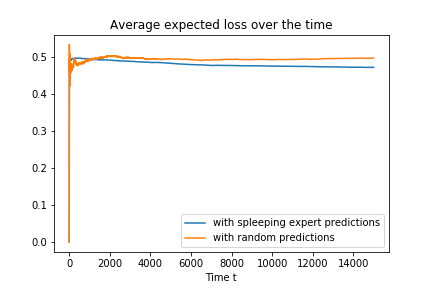
\includegraphics[height=130pt]{image1/image2/VOTES_random_EWA.png}
      \caption{Average loss when playing EWA for $\eta=0.001$, compared with random predictions}
      \label{fig:q7a}
    \end{subfigure}%
    \hspace{2mm}
    \begin{subfigure}{.47\textwidth}
      \centering
      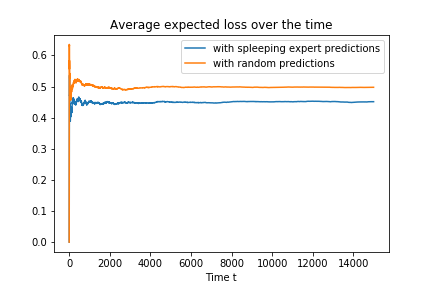
\includegraphics[height=130pt]{image1/image2/VOTES_random_OGD.png}
      \caption{Average loss when playing OGD for $\eta=0.001$, compared with random predictions}
      \label{fig:q7b}
    \end{subfigure}%
    \caption{}
    \end{figure}

EWA produces a slightly better prediction when compared with the average loss of the random prediction. Its accuracy is around 62\%. OGD produces a much better solution in terms of average loss, from the beginning, and that has an accuracy around 60 \%.
	\end{solution}

		\item At each round $t\geq 1$, assume that the algorithms predict the vote $\hat Y_t = 1$ with probability $\hat y_t$ and $0$ otherwise. For each algorithm (for the $\eta$ chosen in question 6(a)), plot its true average loss 
		\begin{equation*}
			\textstyle{\frac{1}{t} \sum_{s=1}^t \indic_{\hat Y_s \neq y_s} \,,}
		\end{equation*}
		according to $t=1,\dots,T$.
		
		\begin{solution}
		\begin{figure}[h!]
    \centering
    \begin{subfigure}{.47\textwidth}
      \centering
      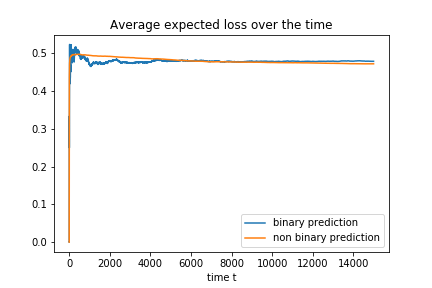
\includegraphics[height=130pt]{image1/image2/VOTES_EWA_bernoulli.png}
      \caption{Average loss when playing EWA for $\eta=0.001$, compared with binary predictions}
      \label{fig:q7a}
    \end{subfigure}%
    \hspace{2mm}
    \begin{subfigure}{.47\textwidth}
      \centering
      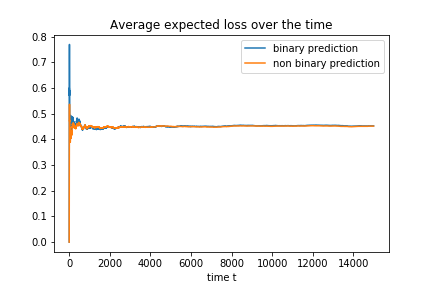
\includegraphics[height=130pt]{image1/image2/VOTES_OGD_bernoulli.png}
      \caption{Average loss when playing OGD for $\eta=0.001$, compared with binary predictions}
      \label{fig:q7b}
    \end{subfigure}%
    \caption{}
    \end{figure}
		\end{solution}
	Even if the true average is a dirac, which is non convex and whose gradient is not bounded, its loss is almost the same as the loss from question 14), for both updates. 

	\end{enumerate}

	\item (optional) Explore different ideas to improve the final performance. For example, you can add new sleeping strategies to be combined or you can perform OGD or EG to estimate the best Bradley Terry model (\url{https://en.wikipedia.org/wiki/Bradley-Terry_model}) on the fly,\dots
\end{enumerate}